\chapter{Two Sample Hypothesis Tests}

\section{Comparing Means with Independent Samples}
\begin{figure}[H]
\centering
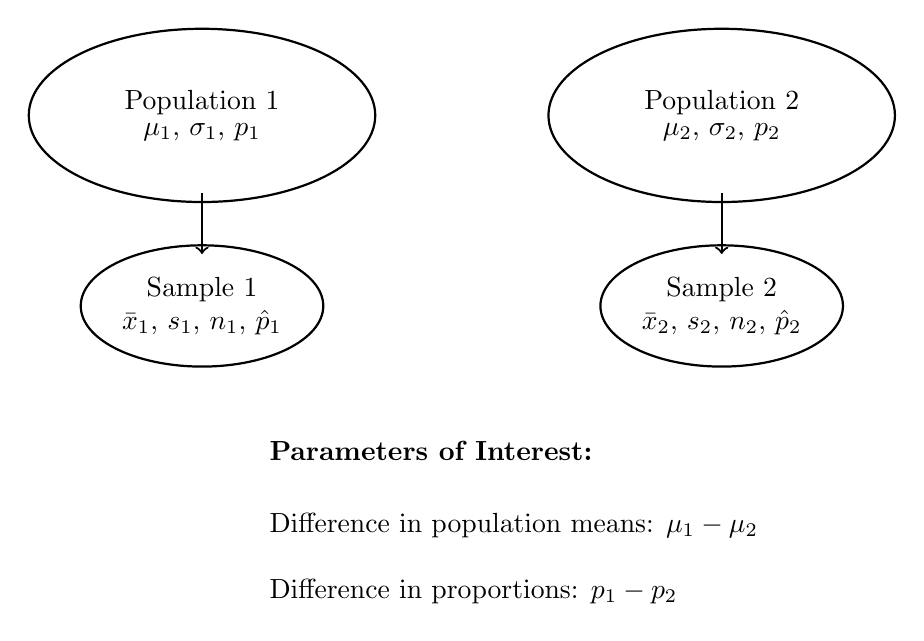
\begin{tikzpicture}[scale=1.1]

% Population 1
\draw[thick] (0,3.5) ellipse (2 and 1);
\node at (0,3.5) {\shortstack{Population 1 \\ $\mu_1$, $\sigma_1$, $p_1$}};

% Sample 1
\draw[thick] (0,1.3) ellipse (1.4 and 0.7);
\node at (0,1.3) {\shortstack{Sample 1 \\ $\bar{x}_1$, $s_1$, $n_1$, $\hat{p}_1$}};

% Arrow from Pop1 to Sample1
\draw[->, thick] (0,2.6) -- (0,1.9);

% Population 2
\draw[thick] (6,3.5) ellipse (2 and 1);
\node at (6,3.5) {\shortstack{Population 2 \\ $\mu_2$, $\sigma_2$, $p_2$}};

% Sample 2
\draw[thick] (6,1.3) ellipse (1.4 and 0.7);
\node at (6,1.3) {\shortstack{Sample 2 \\ $\bar{x}_2$, $s_2$, $n_2$, $\hat{p}_2$}};

% Arrow from Pop2 to Sample2
\draw[->, thick] (6,2.6) -- (6,1.9);

% Parameters of Interest
\node[align=left] at (3.6,-1.2) {
\textbf{Parameters of Interest:} \\\\[2pt]
Difference in population means: $\mu_1 - \mu_2$ \\\\
Difference in proportions: $p_1 - p_2$
};

\end{tikzpicture}
\caption{Structure of Two-Sample Hypothesis Tests}
\end{figure}
\subsection*{Setting Up Hypotheses}

Let $\theta_1$ and $\theta_2$ be the parameters of interest from populations 1 and 2, respectively.

\vspace{0.8em}
\noindent\textbf{1. Interested in whether $\theta_1 > \theta_2$:}
\begin{align*}
H_0\!:~ & \theta_1 = \theta_2 \\
H_a\!:~ & \theta_1 > \theta_2 \\
\text{Equivalent:} \quad & H_0\!:~ \theta_1 - \theta_2 = 0 \qquad H_a\!:~ \theta_1 - \theta_2 > 0
\end{align*}

\vspace{0.8em}
\noindent\textbf{2. Interested in whether $\theta_1 < \theta_2$:}
\begin{align*}
H_0\!:~ & \theta_1 = \theta_2 \\
H_a\!:~ & \theta_1 < \theta_2 \\
\text{Equivalent:} \quad & H_0\!:~ \theta_1 - \theta_2 = 0 \qquad H_a\!:~ \theta_1 - \theta_2 < 0
\end{align*}

\vspace{0.8em}
\noindent\textbf{3. Interested in whether $\theta_1 \ne \theta_2$:}
\begin{align*}
H_0\!:~ & \theta_1 = \theta_2 \\
H_a\!:~ & \theta_1 \ne \theta_2 \\
\text{Equivalent:} \quad & H_0\!:~ \theta_1 - \theta_2 = 0 \qquad H_a\!:~ \theta_1 - \theta_2 \ne 0
\end{align*}
\subsection*{Structure of a Test Statistic}

\noindent
The general structure of a test statistic is:
\[
\text{test statistic} = \frac{\text{(observed statistic)} - \text{(hypothesized value)}}{\text{standard error}}
\]

\bigskip
\noindent\textbf{Common Cases:}
\begin{itemize}
  \item $\sigma$ known: \quad $z = \dfrac{\bar{x} - \mu_0}{\sigma / \sqrt{n}}$
  \item $\sigma$ unknown: \quad $t = \dfrac{\bar{x} - \mu_0}{s / \sqrt{n}}$
  \item Proportions: \quad $z = \dfrac{\hat{p} - p_0}{\sqrt{p_0(1 - p_0)/n}}$
\end{itemize}
\section*{Hypothesis Test on a Difference of Means (\texorpdfstring{$\mu_1 - \mu_2$}{mu1 - mu2})}
\begin{itemize}
\item When $\sigma_1$ and $\sigma_2$ are known:
\end{itemize}
\begin{align*}
H_0&: \mu_1 - \mu_2 = 0 \\
H_a&: \mu_1 - \mu_2 > 0 \quad \text{(or } < 0 \text{, } \ne 0 \text{)}
\end{align*}

\textbf{Test Statistic:}
\[
z = \frac{(\bar{x}_1 - \bar{x}_2) - 0}{\sqrt{\frac{\sigma_1^2}{n_1} + \frac{\sigma_2^2}{n_2}}}
\]

Reference distribution: standard normal (Z distribution).

\textit{Note: This scenario is rare in practice since both population standard deviations $\sigma_1$ and $\sigma_2$ are seldom known.}
\vspace{0.5em}
\begin{itemize}
\item When $\sigma_1$ and $\sigma_2$ are unknown: 
\end{itemize}
\vspace{1.0em}
\textbf{Case 1: Assume equal variances $\sigma_1^2 = \sigma_2^2$}
\vspace{0.5em}
\begin{align*}
H_0&: \mu_1 - \mu_2 = 0 \\
H_a&: \mu_1 - \mu_2 > 0 \quad \text{(or } < 0 \text{, } \ne 0 \text{)}
\end{align*}

\textbf{Test Statistic:}
\[
t = \frac{(\bar{x}_1 - \bar{x}_2) - 0}{s_p \sqrt{\frac{1}{n_1} + \frac{1}{n_2}}}
\]

where the pooled standard deviation is defined as:
\[
s_p^2 = \frac{(n_1 - 1)s_1^2 + (n_2 - 1)s_2^2}{n_1 + n_2 - 2}
\]

Reference distribution: $t$-distribution with $n_1 + n_2 - 2$ degrees of freedom.

(Use this only when equal variances can reasonably be assumed.) \\
\vspace{1.0em}

\noindent \textbf{Case 2: Assume Unequal Variances $\sigma_1^2 \ne \sigma_2^2$ (Welch's t-test)}
\vspace{0.5em}
\begin{align*}
H_0 &: \mu_1 - \mu_2 = 0 \\
H_a &: \mu_1 - \mu_2 > 0 \quad (\text{or } < 0,\ \ne 0)
\end{align*}

\textbf{Test Statistic:}
\[
t^* = \frac{(\bar{x}_1 - \bar{x}_2) - 0}{\sqrt{\frac{s_1^2}{n_1} + \frac{s_2^2}{n_2}}}
\]

Reference distribution: approximately a $t$-distribution.

\vspace{0.5em}
\textit{Degrees of freedom (by hand):}
\[
\min(n_1 - 1,\ n_2 - 1)
\]

\textit{Note:} R uses a more sophisticated approximation for degrees of freedom in this case.
\section*{Comparing Means of Independent Samples (Normal Population Assumptions)}

We should check the assumption that the underlying populations of individual responses are each Normally distributed. Nearly Normal Condition:

\begin{itemize}
  \item We must check this for both groups; a violation for either one violates the condition.
  \item The Normality assumption matters most when sample sizes are very small.
  \item For $n < 10$ in either group, this method should not be used if the histogram or Normality plots show clear skewness.
  \item For $n$’s of 10 or so, a moderately skewed histogram is okay. But, for strongly skewed data or data containing outliers this method should be avoided.
  \item For larger samples $n \geq 20$, data skewness is less of an issue — but, we still need to check if there are any outliers in the data, extreme skewness, and multiple modes.
\end{itemize}
\subsection*{Comparing Two Populations Means: Independent Sampling (Equal Variances Assumed)}

Consider two independent populations with unknown means $\mu_1$ and $\mu_2$, and unknown standard deviations $\sigma_1$ and $\sigma_2$ ($\sigma_1 = \sigma_2$), respectively. We can make an inference about their mean difference $\mu_1 - \mu_2$ by using the difference between their point estimates (sample means): $\bar{Y}_1 - \bar{Y}_2$. When the assumptions and conditions are met,

\[
\frac{(\bar{Y}_1 - \bar{Y}_2) - (\mu_1 - \mu_2)}{S_p \sqrt{\frac{1}{n_1} + \frac{1}{n_2}}}
= \frac{(\bar{Y}_1 - \bar{Y}_2) - (\mu_1 - \mu_2)}{\sqrt{S_p^2 \left[\frac{1}{n_1} + \frac{1}{n_2} \right] }},
\]

can be modelled by a $t(\nu)$ distribution; where $\nu = n_1 + n_2 - 2$ and

\[
S_p^2 = \frac{(n_1 - 1)s_1^2 + (n_2 - 1)s_2^2}{n_1 + n_2 - 2}.
\]
\begin{tcolorbox}[
  colback=yellow!5,
  colframe=yellow!50!black,
  title={Comparing Two Populations Means: Independent Sampling (Equal Variances Assumed) (cont.)},
  sharp corners,
  boxrule=0.4pt,
  width=\textwidth,
  breakable
]

\textbf{Conditions Required for Valid Inference about $\mu_1 - \mu_2$:}

\begin{enumerate}
  \item The two samples are randomly selected in an independent manner from the two target populations.
  \item Both sampled populations have distributions that are approximately Normal.
  \item The population variances are equal (e.g., $\sigma_1 = \sigma_2$).
\end{enumerate}
\end{tcolorbox}
\subsection*{Small-Sample Confidence Interval for $\mu_1 - \mu_2$ (with equal variances)}

\textbf{Parameter:} $\mu_1 - \mu_2$

\vspace{0.5em}

\textbf{Confidence interval} ($\nu = \text{df}$):

\[
(\bar{Y}_1 - \bar{Y}_2) \pm t_{\alpha/2}(\nu) S_p \sqrt{\frac{1}{n_1} + \frac{1}{n_2}},
\]

where $\nu = n_1 + n_2 - 2$ and
\[
S_p^2 = \frac{(n_1 - 1)s_1^2 + (n_2 - 1)s_2^2}{n_1 + n_2 - 2}
\]

(requires that Normal samples are independent and the assumption that $\sigma_1^2 = \sigma_2^2$). The critical value $t_{\alpha/2}(\nu)$ depends on the particular confidence level and the number of degrees of freedom.
\begin{example}
Comparing Two Population Means Managerial Success Indexes for Two Groups (With Equal Variances Assumed)

Behavioural researchers have developed an index designed to measure managerial success. The index (measured on a 100-point scale) is based on the manager’s length of time in the organization and their level within the term; the higher the index, the more successful the manager. Suppose a researcher wants to compare the average index for the two groups of managers at a large manufacturing plant. Managers in group 1 engage in \textbf{high volume of interactions} with people outside the managers’ work unit (such interaction include phone and face-to-face meetings with customers and suppliers, outside meetings, and public relation work). Managers in group 2 \textbf{rarely interact} with people outside their work unit. Independent random samples of 12 and 15 managers are selected from groups 1 and 2, respectively, and success index of each is recorded.

\vspace{1em}

\textbf{Response variable:} Managerial Success Indexes (quantitative, continuous, 0–100 scale)

\textbf{Explanatory variable:} Type of group (nominal categorical: \textit{Group 1 = interaction with outsiders}, \textit{Group 2 = fewer interactions}) 

\vspace{1em}
\noindent\textbf{R Code}
\begin{tcolorbox}[colback=gray!10, colframe=black!45, arc=2mm,
  before skip=4pt, after skip=4pt]
\begin{verbatim}
# Importing data file into R
success = read.csv(file = "success.csv", header = TRUE);

# Getting names of variables
names(success);

# Seeing first few observations
head(success);

# Attaching data file
attach(success);
\end{verbatim}
\end{tcolorbox}

\noindent\textbf{R Code}
\begin{tcolorbox}[colback=gray!10, colframe=black!45, arc=2mm,
  before skip=4pt, after skip=4pt]
\begin{verbatim}
## [1] "Success_Index" "Group"
##   Success_Index Group
## 1            65     1
## 2            66     1
## 3            58     1
## 4            70     1
## 5            78     1
## 6            53     1
\end{verbatim}
\end{tcolorbox}
\noindent\textbf{R code (Descriptive Statistics)}
\begin{tcolorbox}[colback=gray!10, colframe=black!45, arc=2mm,
  before skip=4pt, after skip=4pt]
\begin{verbatim}
# loading library mosaic
library(mosaic)

favstats(Success_Index ~ Group)
\end{verbatim}
\end{tcolorbox}

\noindent\textbf{R Code (Descriptive Statistics)}
\begin{tcolorbox}[colback=gray!10, colframe=black!45, arc=2mm,
  before skip=4pt, after skip=4pt]
\begin{verbatim}
## .group min   Q1 median   Q3 max     mean       sd  n
##       1  53 62.25  65.50 69.25  78 65.33333 6.610368 12
##       2  34 42.50  50.00 54.50  68 49.46667 9.334014 15
\end{verbatim}
\end{tcolorbox}

\noindent\textbf{R Code (Descriptive Statistics)}
\begin{tcolorbox}[colback=gray!10, colframe=black!45, arc=2mm,
  before skip=4pt, after skip=4pt]
\begin{verbatim}
summary(Success_Index[Group == 1]);
length(Success_Index[Group == 1]);
sd(Success_Index[Group == 1]);

summary(Success_Index[Group == 2]);
length(Success_Index[Group == 2]);
sd(Success_Index[Group == 2]);
\end{verbatim}
\end{tcolorbox}

Note: Group 1 = “interaction with outsiders” and Group 2 = “fewer interactions”.
% --- continuation inside the same example environment ---

\noindent\textbf{R Output}
\begin{tcolorbox}[colback=gray!10, colframe=black!45, arc=2mm,
  before skip=4pt, after skip=4pt]
\begin{verbatim}
##  Min.  1st Qu.  Median    Mean  3rd Qu.    Max. 
##  53.00   62.25   65.50   65.33   69.25   78.00 
## [1] 12
## [1] 6.610368

##  Min.  1st Qu.  Median    Mean  3rd Qu.    Max. 
##  34.00   42.50   50.00   49.47   54.50   68.00 
## [1] 15
## [1] 9.334014
\end{verbatim}
\end{tcolorbox}

\vspace{0.5em}
\noindent\textbf{Nearly Normal Condition (Group 1: “interaction with outsiders”):}
\begin{tcolorbox}[colback=gray!10, colframe=black!45, arc=2mm,
  before skip=4pt, after skip=4pt]
\begin{verbatim}
stem(Success_Index[Group == 1]);
\end{verbatim}
\end{tcolorbox}

\noindent\textbf{R Output}
\begin{tcolorbox}[colback=gray!10, colframe=black!45, arc=2mm,
  before skip=4pt, after skip=4pt]
\begin{verbatim}
## 
##  The decimal point is 1 digit(s) to the right of the |
## 
##  5 | 38
##  6 | 0335689
##  7 | 018
\end{verbatim}
\end{tcolorbox}

\vspace{0.5em}
\noindent\textbf{Nearly Normal Condition (Group 2: “fewer interactions”):}
\begin{tcolorbox}[colback=gray!10, colframe=black!45, arc=2mm,
  before skip=4pt, after skip=4pt]
\begin{verbatim}
stem(Success_Index[Group == 2]);
\end{verbatim}
\end{tcolorbox}

\noindent\textbf{R Output}
\begin{tcolorbox}[colback=gray!10, colframe=black!45, arc=2mm,
  before skip=4pt, after skip=4pt]
\begin{verbatim}
## 
##  The decimal point is 1 digit(s) to the right of the |
## 
##  3 | 46
##  4 | 22368
##  5 | 023367
##  6 | 28
\end{verbatim}
\end{tcolorbox}

\vspace{0.5em}
\noindent\textbf{Nearly Normal Condition (Group 1: “interaction with outsiders”):}
\begin{tcolorbox}[colback=gray!10, colframe=black!45, arc=2mm,
  before skip=4pt, after skip=4pt]
\begin{verbatim}
qqnorm(Success_Index[Group == 1]);
qqline(Success_Index[Group == 1]);
\end{verbatim}
\end{tcolorbox}
\begin{figure}[H]
\centering
\includegraphics[width=0.6\textwidth]{section14.1/images/qqplot_group1.pdf}
\caption{Q-Q Plot for Group 1: Interaction with Outsiders}
\label{fig:qqplot-group1}
\end{figure}
\vspace{0.5em}
\noindent\textbf{Nearly Normal Condition (Group 2: “fewer interactions”):}
\begin{tcolorbox}[colback=gray!10, colframe=black!45, arc=2mm,
  before skip=4pt, after skip=4pt]
\begin{verbatim}
qqnorm(Success_Index[Group == 2]);
qqline(Success_Index[Group == 2]);
\end{verbatim}
\end{tcolorbox}
\noindent
\begin{minipage}{\textwidth}
\centering
\includegraphics[width=0.6\textwidth]{section14.1/images/qqplot_group2.pdf}
\vspace{-0.5em}

\captionof{figure}{Q-Q Plot for Group 2: Fewer Interactions}
\label{fig:qqplot-group2}
\end{minipage}

\vspace{1.00em}

\noindent\textbf{Nearly Normal Condition:}
\begin{tcolorbox}[colback=gray!10, colframe=black!45, arc=2mm,
  before skip=4pt, after skip=4pt]
\begin{verbatim}
boxplot(Success_Index ~ Group, col = c("red", "blue"))
\end{verbatim}
\end{tcolorbox}
\noindent
\begin{minipage}{\textwidth}
\centering
\includegraphics[width=0.55\textwidth]{section14.1/images/boxplot_success_index.pdf}
\vspace{-0.5em}

\captionof{figure}{Boxplot of Success Index by Group}
\label{fig:boxplot-success}
\end{minipage}
\vspace{-1,00em}

\noindent\textbf{Boxplot with \texttt{ggplot2}:}
\begin{tcolorbox}[colback=gray!10, colframe=black!45, arc=2mm,
  before skip=4pt, after skip=4pt]
\begin{verbatim}
# loading library;
library(ggplot2);

# converting a numeric variable into factor (categorical data)
group <- factor(Group);

# bp: just a name (not code) to store boxplots;
bp <- ggplot(success,
             aes(x = group, y = Success_Index, fill = group));

our.labs <- c("Interaction with Outsiders", "Fewer Interactions");

bp +
  geom_boxplot() +
  scale_x_discrete(labels = our.labs);
\end{verbatim}
\end{tcolorbox}
\begin{figure}[H]
\centering
\includegraphics[width=0.6\textwidth]{section14.1/images/boxplot_ggplot2.pdf}
\caption{Boxplot of Success Index by Group using ggplot2}
\label{fig:boxplot-ggplot}
\end{figure}
\noindent\textbf{Checking the Assumptions and Conditions}

\vspace{0.5em}

\noindent\textbf{Independent Group Assumption:} The success index in group 1 is unrelated to the success index in group 2.

\noindent\textbf{Randomization Condition:} The 27 managers were randomly and independently selected (12 for group 1, and 15 for group 2).

\noindent\textbf{Nearly Normal Condition:} The two boxplots of success indexes do not show skewness; the two stemplots/histograms of success indexes are unimodal, fairly symmetric and approximately bell-shaped. Q–Q plots also suggest the normality assumption is reasonable.

\noindent\textbf{Equal Variances Assumption:} The two boxplots of success indexes appear to have the same spread; thus, the samples appear to have come from populations with approximately the same variance.

\vspace{0.5em}

Since the conditions are satisfied, it is appropriate to construct a $t$ confidence interval with\\
$df = 12 + 15 - 2 = 25$. \\

\noindent\textbf{From the data, the following statistics were calculated:}

\[
\begin{aligned}
n_1 &= 12 &\quad n_2 &= 15 \\
\bar{x}_1 &= 65.33 &\quad \bar{x}_2 &= 49.47 \\
s_1^2 &= 6.61^2 &\quad s_2^2 &= 9.33^2
\end{aligned}
\]

\vspace{1em}
\noindent\textbf{The pooled variance estimator is:}

\[
s_p^2 = \frac{(n_1 - 1)s_1^2 + (n_2 - 1)s_2^2}{n_1 + n_2 - 2} 
= \frac{(12 - 1)(6.61^2) + (15 - 1)(9.33^2)}{12 + 15 - 2}
= 67.97
\]

\vspace{1em}
\noindent\textbf{The number of degrees of freedom is:}
\[
\nu = n_1 + n_2 - 2 = 12 + 15 - 2 = 25
\]

\vspace{1em}
\noindent\textbf{Two-sample t-test (Student’s t-test) for the Difference Between Means $\mu_1 - \mu_2$:}

Is there evidence to suggest that the mean success index differs between the two groups?

\vspace{1em}
\noindent\textbf{1. State Hypotheses:}
\[
\begin{aligned}
H_0 &: \mu_1 = \mu_2 \quad \text{or} \quad H_0 : \mu_1 - \mu_2 = 0 \\
H_a &: \mu_1 \ne \mu_2 \quad \text{or} \quad H_a : \mu_1 - \mu_2 \ne 0
\end{aligned}
\]

\vspace{1em}
\noindent\textbf{2. Test Statistic:}
\[
t^* = \frac{\bar{x}_1 - \bar{x}_2}{\sqrt{\frac{s_p^2}{n_1} + \frac{s_p^2}{n_2}}}
= \frac{65.33 - 49.47}{\sqrt{\frac{67.97}{12} + \frac{67.97}{15}}}
= 4.97
\]

\vspace{1em}
\noindent\textbf{3. P-value:}

Using table:
\[
\text{df} = 25 \quad \Rightarrow \quad \text{P-value} < 2(0.005)
\]

Using R:
\begin{tcolorbox}[colback=gray!10, colframe=black!45, arc=2mm, before skip=4pt, after skip=4pt]
\begin{verbatim}
# One way:
2*(1 - pt(4.97, df = 25));

# Another way:
2 * pt(4.97, df = 25, lower.tail = FALSE);
\end{verbatim}
\end{tcolorbox}

Both methods return:
\[
\text{P-value} \approx 4.03 \times 10^{-5}
\]
\vspace{1em}
\noindent\textbf{4. Conclusion.}

Since the P-value is very small, we have strong evidence to indicate that there is a difference in mean success index between group~1 and group~2.

\vspace{0.5em}
\noindent\textbf{Note.} As a follow-up, we could find a 95\% CI for $\mu_1 - \mu_2$ to estimate this difference. Then, we could provide an estimate of how much higher the mean success index for group~1 is.


\end{example}


